% !TeX root = ../main.tex
% Add the above to each chapter to make compiling the PDF easier in some editors.

\chapter{Future Work}\label{chapter:future_work}

Intel Trust Domain Extensions is Intel's upcoming Confidential Computing technology.
Similar to other technologies, such as AMD SEV-SNP or ARM CCA, it is based on hardware-isolated virtual machines. These so-called Trust Domains (TDs) are based on a combination between Intel Virtual Machine Extensions (VMX), multi-key, total-memory-encryption (MKTME) and a software module protected by the CPU. \parencite{tdx_paper} 

The digitally signed TDX module is thereby executed in a new high-privileged processor mode called Secure-Arbitration Mode (SEAM) and is hosted in dedicated memory space.
Because this memory range is protected, it can only be accessed from other software executing inside the same region. Any access from outside is aborted. 
Since the TDX module acts as an intermediary control instance between the secure VMs and the HV, it provides an interface for creation, managing and loading of TDs.

\begin{figure}
	\begin{center} 
		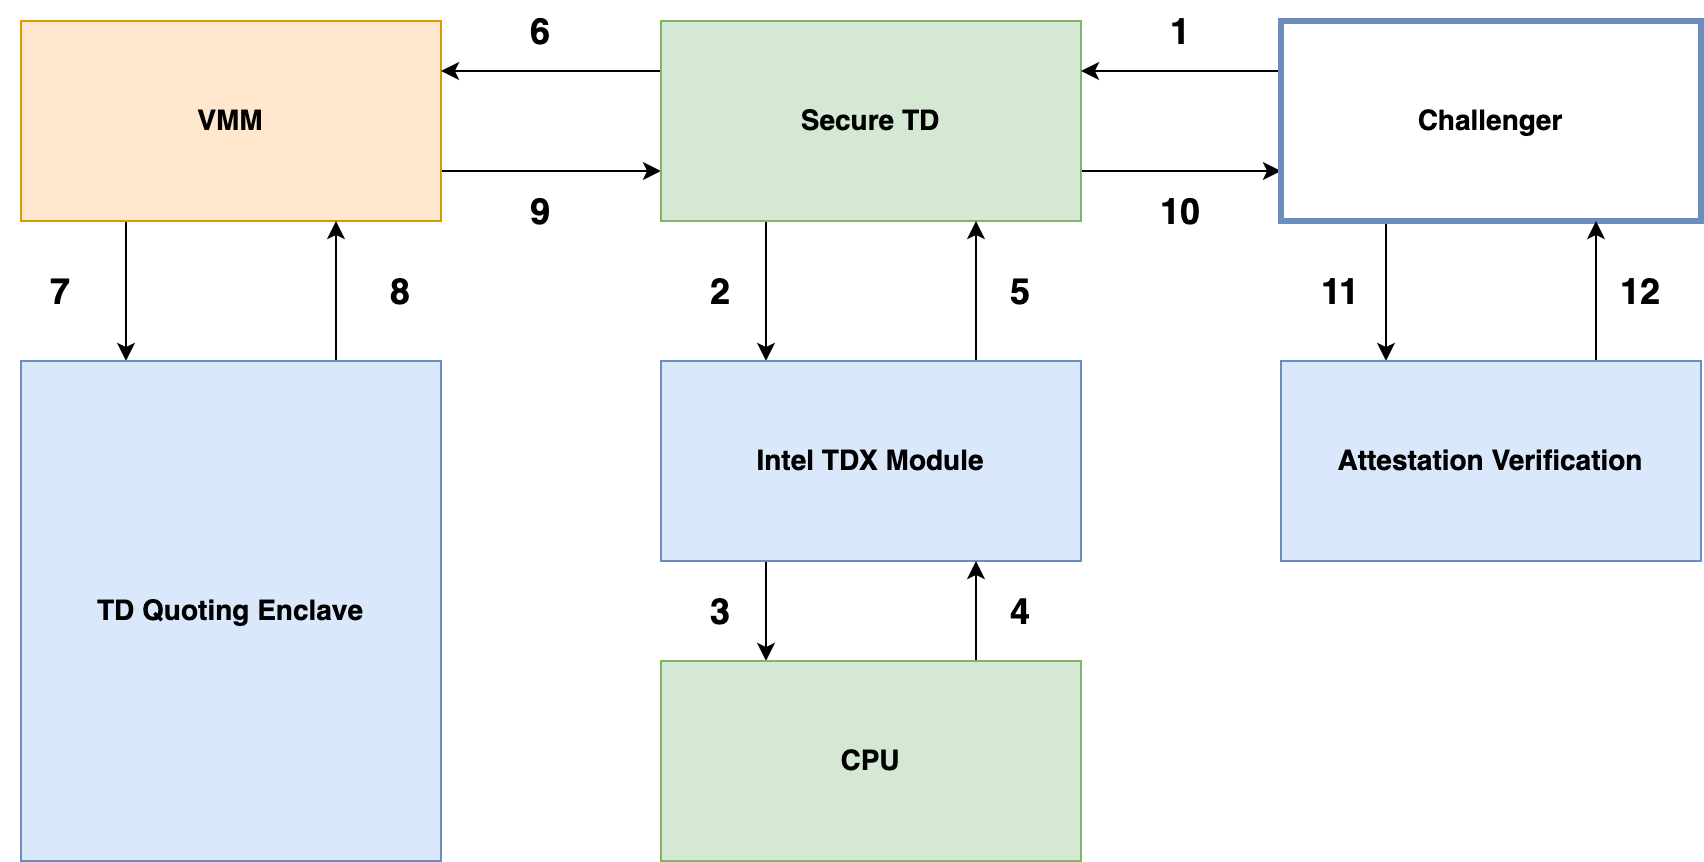
\includegraphics[width=1.0\linewidth]{figures/tdx.drawio.png}
	\end{center}
	\caption{TDX attestation flow \cite{tdx_paper}} 
	\label{tdx-attesation}
\end{figure}

The attestation workflow of Intel TDX is heavily based on SGX Enclaves. Figure \ref{tdx-attesation} shows the process of generating a report. During the creation of a Trusted Domain (TD), special measurement registers receive the initial measurement data from the TCB. Subsequently, these measurements can be expanded during runtime using additional registers. When a request is sent by a challenger, the TDX module asks the CPU to produce a report for the corresponding VM and protect it with a MAC.
This report is then forwarded to the HV, which converts the report to a remote attestation report (quote) by using the TDX Quoting Enclave, which is essentially the SGX QE. Finally the quote is then sent back to the challenger for verification. \cite{TDX_comparison_quartet}

The basic report structure from a TDX report is similar to the one of SGX with the main difference being the report body. This has the advantage that the report validation is similar to that of SGX reports. 
The DCAP library already provides functions for quote generation and verification that reuse many functions of the SGX implementation. Also in the CMC some functions of the current SGX implementation can be reused, various parsing functions and even the function to verify the Quote Signature Data structure. Nevertheless there are some values which differ and new values which have to be checked. 

Since TDX, as a VM-based TEE, supports the execution of multiple processes, the implementation of the quote generation is much easier than for SGX. Similar to SNP, the CMCD, estserver and the calling application can all be executed within the VM, which simplifies the creation of an attested TLS connection to another TEE.
At the time of writing no publicly availble TDX hardware exists so far. As soon as this becomes available, it can also be implemented in the framework. 